\paragraph{Regression Trees}
\subparagraph{Predication via Stratification of the feature space }
\begin{itemize}
	\item \tB{We divide the predictor space (the set of possible 
		values for $\prth{X}{j}{p}$) into $J$ distinct and non
		overlapping regions $\prth{R}{k}{J}$.}
	\item \sB{For every observation that falls into the region
		$R_{j}$ we make the same prediction, which is simply
		the mean of the response values} for the training 
		observation in $R_{j}$
\end{itemize}
Theoretically the regions could have any shape, however we choose to
divide the predictor space into high-dimensional rectangles (boxes).
\tB{The goal is to find $\prth{R}{k}{J}$ that minimize the RSS given by
:}
\begin{center}
\encV{
$\su{{k=1}}{J}\su{{i\in R_{k}}}{}\left(y_{i}-\hat{y}_{R_{k}}\right)^{2}$}
\end{center}
where $\hat{y}_{R}$, is the mean response for the training observations
within the $k^{th}$ box.
It is computationally infeasible to consider every possible partition
of the feature space into $J$ boxes.\\
For this reason, we take an approach which is:
\begin{itemize}
	\item \textbf{\emph{top-down}}: \sB{it begins at the top of the
		tree} (at which point all observations belong to a 
		single region) \sB{and then successively splits the 
		predictor space.}
	\item \textbf{\emph{greedy}}: at each step of the tree-building
		process, the best split is made at that particular step
\end{itemize}
It is known as \tR{\emph{recursive binary splitting}}\\

We select the predictor $X_{j}$ and the cutpoint $s$ such that 
splitting the predictor space into the regions $\left\{X|X_{j}<s\right\}$ (``\emph{the region of predictor space in which} $X_{j}$ \emph{takes
on a value less than} $s$'') and $\left\{X|X_{j}>s\right\}$ leads to the greatest possible 
reduction in RSS.
For any $j$ and $s$ \sB{we define the pair of half-planes}:
\encB{$
\begin{cases}
	R_{1}(j,s)=\left\{ X|X_{j}<s \right\}\\
	R_{2}(j,s)=\left\{ X|X_{j}>s \right\}
\end{cases}$}
and \sB{we seek the value of $j$ and $s$ that minimize}:

\begin{center}
\enc{
	$\su{{i:x_{i}\in R_{1}(j,s)}}{}\left( y_{i}-\hat{y}_{R_{1}} \right)^{2} + \su{{i:x_{i}\in R_{2}(j,s)}}{}\left( y_{i}-\hat{y}_{R_{2}} \right)^{2}$}
\end{center}
where \tB{$\hat{y}_{R_{1}} = ave\left(y_{i}|x_{i}\in R_{1}(j,s)\right)$} is the mean response for the 
training observations in $R_{1}(j,s)$  

\subparagraph{Tree Pruning}
A smaller tree with fewer splits (fewer regions $\prth{R}{i}{J}$) might
lead to lower variance and better interpretation at the cost of a 
little bias.\\ A better strategy is to grow a very large tree $T_{0}$,
and then \emph{prune} it back in order to obtain a \emph{subtree}.\\
Rather than considering every possible subtree, \sB{we consider a
sequence of trees indexed by a nonnegative tuning parameter $\alpha$}.

\paragraph{Algorithm: Building a Regression Tree}
\begin{enumerate}
	\item \tB{Use recursive binary splitting} to grow a large tree on 
		the training data, \sB{stopping only when each terminal
		node has fewer than some minimum number of observations}
	\item Apply cost complexity pruning to the large tree in order
		to obtain a sequence of subtrees, as a function of 
		$\alpha$
	\item \tB{Use $K$-fold cross-validation to choose $\alpha$}.
		That is divide the training observations into $K$-folds.
		\begin{enumerate}[label=\Alph*]
			\item \sB{Repeat steps 1 and 2 on all but $k^{
				th}$ fold} of the training data.
			\item Evaluate the mean squared prediction 
				error on the data in the left-out 
				$k^{th}$, as a function of $\alpha$
		\end{enumerate}
		Average the results for each value of $\alpha$, and
		pick $\alpha$ to minimize the average error.
	\item Return the subtree from Step 2 that correspond to the
		chosen value of $\alpha$
\end{enumerate}

For each value of $\alpha$ there corresponds a subtree $T\subset T_{0}$
such that:
\begin{center}
	\enc{ $
	\su{{m=1}}{|T|}\su{{i:x_{i}\in R_{m}}}{}\left( y_{i}-\hat{y}_{Rm} \right)^{2} + \alpha|T| $}
\end{center}
is as small as possible. \tB{$|T|$ indicates the number of terminal nodes of the tree $T$.}

\begin{python}
import sklearn
from sklearn import tree

X = [[0, 0], [2, 2]] 
y = [0.5, 2.5]
reg = tree.DecisionTreeRegressor()
reg = reg.fit(X, y) 
print(reg.score(X, y))
\end{python}

\paragraph{Classification Trees}
The \tB{classification error rate} is simply the fraction of the training
observations in that region that do not belong to the most common 
class:
$E=1-\max\limits_{k}(\hat{p}_{mk})$
Here $\hat{p}_{mk}$ represents the proportion of training 
observation in the $m^{th}$ region are from the $k^{th}$ class, \tB{$\hat{p}_{mk}=\dfrac{1}{N_{m}}
\su{{x_{i}\in R_{m}}}{}I(y_{i}=k)$}.\\
It turns out that classification error is not sufficiently sensitive 
for tree-growing, and in practice 2 other measures are preferable.\\
The Gini index is defined by
$$
G=\su{{k=1}}{K}\hat{p}_{mk}(1-\hat{p}_{mk})
$$\\
The \tB{entropy} given by:
\encB{$D = -\su{{k=1}}{K}\hat{p}_{mk}\ln\left( \hat{p}_{mk} \right)$}\\
The entropy \sB{will take on a value near zero if the $\hat{p}_{mk}$'s are
all near zero or near one}.\\ Therefore, like the Gini index, the 
entropy will take on a small value if the $m^{th}$ node is pure.\\

Any of these three approaches might be used when \emph{pruning} \sB{the
tree, but the classification error rate is preferable if prediction
accuracy of the final pruned tree is the goal}.

\begin{python}
import sklearn
from sklearn import tree

X, y = load_iris(return_X_y=True)
clf = tree.DecisionTreeClassifier()
clf = clf.fit(X, y) 
print(clf.score(X, y))
tree.plot_tree(clf)
\end{python}
\paragraph{Advantages and Disadvantages of Trees}
\begin{itemize}
	\item[\tV{+}] They are very easy to explain to people.
		easily interpreted.
	\item[\tV{+}] Trees can be displayed graphically, and are 
		easily interpreted
	\item[\tV{+}] Trees can easily handle qualitative predictors 
		without the need to create dummy variables.
	\item[\tR{-}] Trees generally do not have the same level of
		predictive accuracy as some of the other regression
		and classification approaches.
	\item[\tR{-}] Trees can be non-robust, a small change in the 
		data can cause a large change in the final estimated
		tree.
\end{itemize}

\paragraph{PRIM: Bump Hunting}
Tree-based methods (for regression) partition the feature space into box-shaped regions, to try to
make the response averages in each box as different as possible.\\
The \tB{Patient Rule Introduction Method} (PRIM) also finds boxes in the feature space, but seeks 
boxes in which the response average is high. Hence it looks for maxima in the target function.
PRIM also differs from tree-based partitioning methods in that the box definition are not 
described by a binary tree.
This makes interpretation of the collection of rules more difficult; however, by removing the binary
tree constraint, the individual rules are often simpler.
\subparagraph{Example}
There are 200 data points uniformely distributed over the unit square. The color-coded plot indicates
the response $Y=
\begin{cases}
	1\text{ (red), }0.5<X_{1}<0.8\text{ and }0.4<X_{2}<0.6\\
	0\text{ (blue), otherwise}
\end{cases}$\\
The panel shows the successive boxes found by the top-down peeling procedure, peeling off a 
proportion $\alpha=0.1$ of the remaining data points at each stage.\\
After the top-down sequence is computed, PRIM reverses the process, expanding along any edges, if 
such an expansion increases the box mean, this called \emph{pasting}.
\begin{figure}[H]
	\begin{center}
		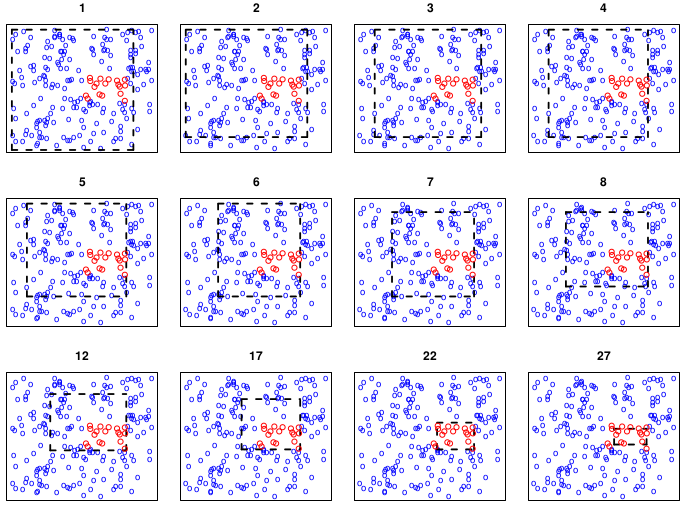
\includegraphics[width=.7\textwidth]{./chap/1chap/7sec/images/6_prim.png}
	\end{center}
	\caption{The procedure starts with a rectangle (broken black lines) surronding all of the 
	data, and then \tB{peels away points along one edge by a prespecified amout in order to
	maximize the mean of the points remaining in the box}. The iteration number is indicated at 
	the top of each panel.}
	\label{fig:6_prim}
\end{figure}
\subparagraph{Patient Rule Induction Method}
\begin{enumerate}
	\item \sB{Start with all of the training data}, and a maximal box containing all of the data
	\item Consider shrinking the box by compressing one face, so as to \sB{peel off the 
		proportion $\alpha$ of observations having either the highest values of a 
		predictor $X_{j}$ or the lowest}. Choose the peeling that produces the highest
		response mean in the remaining box. (Typically $\alpha=0.05$ or 0.10) 
	\item Repeat \sB{step 2 until some minimal number of observation remain in the box}, (say 10).
	\item Expand the box along any face, as long as the resulting box mean increases.
	\item Step 1-4 give a sequence of boxes, with different numbers of observation in each
		box. \sB{Use cross-validation to choose a member of the sequence.} Call the box
		$B_{1}$
	\item Remove the data in box $B_{1}$ from the dataset and repeat steps $2-5$ to obtain
		a second box, and continue to get as many boxes as desired.
\end{enumerate}
This produces a sequence of boxes $\prth{1}{l}{k}$, each box is defined by a set of rules involving
a subset of predictors like: 
$\begin{cases}
	a_{1}\leq X_{1}\leq b_{1}\\
	a_{3}\leq X_{3}\leq b_{3}
\end{cases}$

\paragraph{MARS: Multivariate Adaptive Regression Splines}
MARS is an \tB{adaptive procedure for regression, and is well suited for high-dimensional problems}.
MARS uses expansions in piecewise linear basis functions of the form $(x-t)_{+}$, $(t-x)_{+}$
\begin{center}
	$(x-t)_{+} = \begin{cases} x-t \Leftarrow x>t\\ 0\Leftarrow x\leq t\end{cases}$ and 
$(t-x)_{+} = \begin{cases} t-x \Leftarrow x<t\\ 0\Leftarrow x\geq t\end{cases}$
\end{center}
Therefore, the collection of basis function is: 
\begin{center}
	\encB{$ \mathcal{C}=\left\{(X_{j}-t)_{+}, (t-X_{j})_{+}|\in\left\{x_{ij}\right\}_{1\leq i\leq N}\right\}_{1\leq j\leq p}$}
\end{center}
Thus the model has the form 
\begin{center}
	\enc{$ f(X)=\beta_{0}+\su{{m=1}}{M}\beta_{m}h_{m}(X)$}
\end{center}
where each \sB{$h_{m}(X)$ is a function in $\mathcal{C}$} or a product of 2 or more such functions.\\
Given a choice for the $h_{m}$, the coefficient $\beta_{m}$ are estimated by minimizing the residual
sum-of-squares, that is, by standard linear regression.\\
At each stage we consider as a new basis function pari all products of a function $h_{m}$ in the 
model set $\mathcal{M}$ with one of the reflected pairs in $\mathcal{C}$\\
We add to the model $\mathcal{M}$ the term of the form:
\begin{center}
$\hat{\beta}_{M+1}h_{l}(X)\times(X_{j}-t)_{+}+\hat{\beta}_{M+2}h_{l}(X)\times(t-X_{j})_{+}, h_{l}\in
\mathcal{M}$
\end{center}
that produces the largest decrease in training error. Here $\hat{\beta}_{M+1}$ and $\hat{\beta}_{M+2
}$ are coefficients estimated by least squares, along with all other $M+1$ coefficient in the model.
\begin{python}
import pyearth
from pyearth import Earth

model_mars = Earth()
model_mars.fit(X, y)
\end{python}
\subparagraph{Example}
At the first stage we consider adding to the model a function of the form $\beta_{1}\left(X_{j}-t
\right)_{+}+\beta_{2}\left(t-X_{j}\right)_{+}; t\in\left\{x_{ijj}\right\}$ since multiplication by
the constant function just produces the functdion itself.\\
Suppose the best choice is $\hat{\beta}_{1}\left(X_{2}-x_{72}\right)_{+}+\hat{\beta}_{2}\left(x_{72}-X_{2}\right)_{+}$.\\
Then this pair of basis functions is added to the set $\mathcal{M}$ and the next stage we consider
including a pair of products the form:
$h_{m}(X)\times\left(X_{j}-t\right)_{+}\text{ and }h_{m}(X)\left(t-X_{j}\right)_{+}, t\in\left\{
x_{ij}\right\}$
where we have the choices:
\begin{align*}
	h_{0}(X) &= 1\\
	h_{1}(X) &= \left(X_{2}-x_{72}\right)_{+}\\
	h_{0}(X) &= \left( x_{72}-X_{2} \right)
\end{align*}

\subparagraph{Cross-validation}
One could use cross-validation to estimate the optimal value of $\lambda$, but for computational
savings the MARS procedure instead uses generalized cross-validation:
$$ GCV(\lambda) = \dfrac{\su{{i=1}}{N}\left(y_{i}-\hat{f}_{\lambda}(x_{i})\right)^{2}}{
\left(1-\frac{M(\lambda)}{N}\right)^{2}}$$
The $M(\lambda)$ is the effective number of parameters in the model: this accounts both for the
number of parameters used in selecting the optimal positions of the knots. 
